\section{Introduction and Planning}

The web interface and it's supporting software are crucial components that enable users to interact with Tiberius remotely. It is also the enabler for mission planning and execution. These concepts are further discussed in Section  \ref{sec:web_design_missions}.

Figure \ref{fig:web-interface-communication} illustrates the communication relationships between the Tiberius robots and the web applications, and gives a clear overview of our web components. The figure illustrates two Tiberius robots (left), an instance of the web interface (top right) and an android application (bottom left). In this configuration, both the web interface and android application can communicate with either robot.

\begin{figure}[!htb]
\begin{center}
\includegraphics[width=10cm]{web_interface_comms.png}
\end{center}
\caption{Web Interface Communication}
\label{fig:web-interface-communication}
\end{figure}


Remaining with Figure \ref{fig:web-interface-communication}, everything is encapsulated within the \gls{VPN}. This is a network with virtual bridges to allow one network to exist but in multiple physical locations. For a more detailed description of our \gls{VPN}, refer to section \ref{sec:comms_theory_vpn}. All robots and web applications must be connected to our \gls{VPN} to allow communication.

Multiple robots can exist on our network but at the same time each robot must be assigned a static IP address. In theory, multiple instances of the web interface can exist on the same network, although we only require one for our purposes. Many applications such as the Android Application can also be active on the network at once.

All communication between devices is in the form of \gls{HTTP} \gls{POST} requests/responses. The security benefits of this message type are described in section \ref{sec:web_subsystem_overview}.

Figure \ref{fig:api-interaction} illustrates the existing functions of the \gls{controlapi}, as well as unimplemented functions that could be considered for future work. Possible future projects are described in-depth in section \ref{sec:web_future_work}.
\begin{figure}[!htb]
\begin{center}
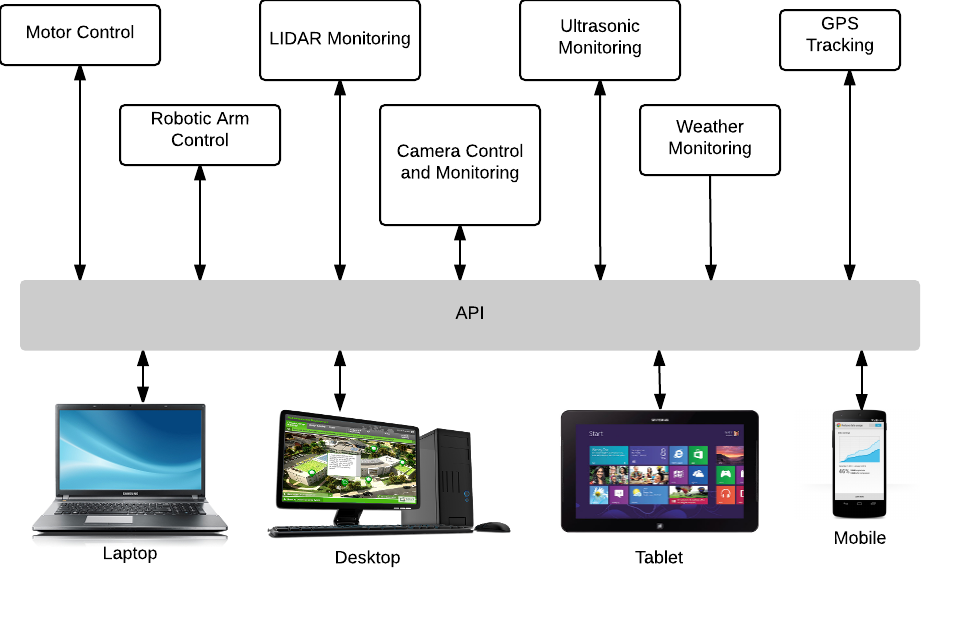
\includegraphics[width=10cm]{api_diagram.png}
\end{center}
\caption{API Interaction}
\label{fig:api-interaction}
\end{figure}

The \gls{controlapi} is a server application that runs on each Tiberius robot, allowing authenticated devices to communicate with it. The \gls{controlapi} may also be refereed to as the 'API' or 'Tiberius API', from herein. The \gls{controlapi} is 'supporting software', as it supports the operation of the web interface, by handling it's \gls{HTTP} \gls{POST} messages. Like most application on Tiberius, the \gls{controlapi} is written in Python, so can interact with Tiberius's other software extremely easily, this integration with existing software is crucial to allow the \gls{controlapi} to operate Tiberius. The \gls{controlapi} provides the following to compatible applications:

\begin{itemize}
\item Provides access to Tiberius' basic motor control functions, allowing external applications to tele-operate the vehicle.

\item Similarly, the robotic arm can be tele-operated by interfacing with the \gls{controlapi}.

\item Allows external applications to make queries to Tiberius' in-memory database. These are controlled queries, there is no direct SQL statement support. This is a security measure preventing misuse of the API's database access.

\item Supporting applications can provide authenticated start, pause and stop commands to control tasks. These are used during missions when Tiberius reaches a waypoint with tasks assigned to it.

\item The point-to-point algorithm (discussed in section \ref{sec:nav_design_p2p}) can be started from the \gls{controlapi}, this is used during missions to navigate from waypoint to waypoint.

\end{itemize}

% \begin{lstlisting}[caption=HTTP POST Example, label=amb]
% Name=Gareth+Wylie&Age=24&Formula=a+%2B+b+%3D%3D+13%25%21
% \end{lstlisting}